\documentclass{article}
\usepackage{pgfplots}
\pgfplotsset{compat=1.18}

\begin{document}

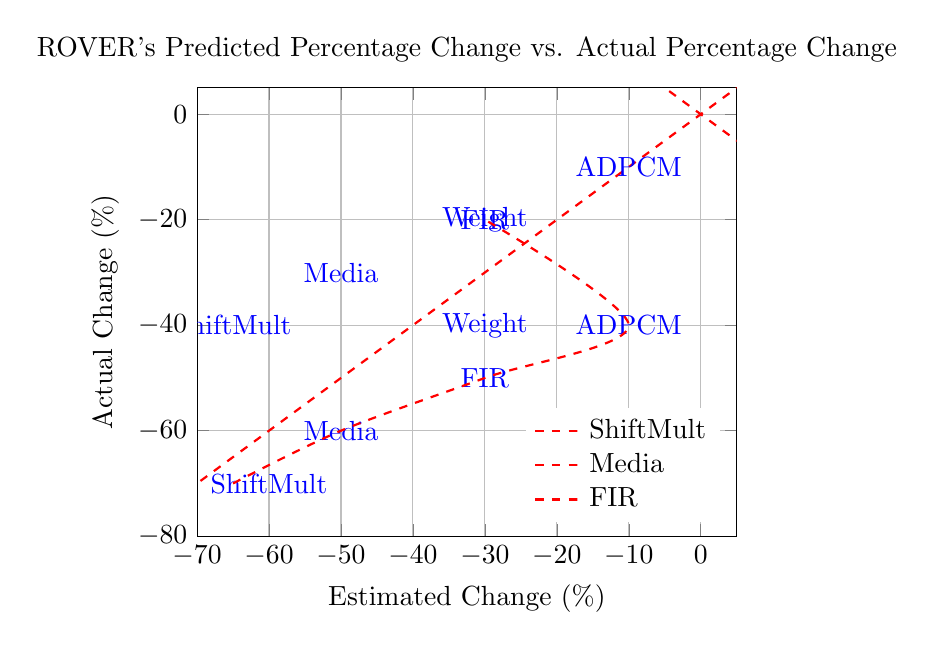
\begin{tikzpicture}
    \begin{axis}[
        title={ROVER's Predicted Percentage Change vs. Actual Percentage Change},
        xlabel={Estimated Change (\%)},
        ylabel={Actual Change (\%)},
        xmin=-70, xmax=5,
        ymin=-80, ymax=5,
        xtick={-70,-60,...,5},
        ytick={-80,-60,...,5},
        grid=major,
        legend pos=south east,
        legend cell align=left,
        legend style={draw=none},
        samples=2,
        smooth,
        domain=-90:90,
        no markers,
        % Style for red lines
        every axis plot post/.append style={
            mark=none,
            color=red,
            dashed,
            thick
        },
    ]
        % Red line for synthesis noise window
        \addplot[no markers] {x};
        \addplot[no markers] {-x};
        
        \node at (-65,-40) [blue] {ShiftMult};
        \node at (-50,-30) [blue] {Media};
        \node at (-30,-20) [blue] {FIR};
        \node at (-10,-10) [blue] {ADPCM};
        \node at (-30,-40) [blue] {Weight};
        
        \node at (-60,-70) [blue] {ShiftMult};
        \node at (-50,-60) [blue] {Media};
        \node at (-30,-50) [blue] {FIR};
        \node at (-10,-40) [blue] {ADPCM};
        \node at (-30,-20) [blue] {Weight};
        
        % Data points
        \addplot [mark=*] coordinates {
            (-65, -70)
            (-50, -60)
            (-30, -50)
            (-10, -40)
            (-30, -20)
        };
        
        \legend{ShiftMult, Media, FIR, ADPCM, Weight}
    \end{axis}
\end{tikzpicture}

\end{document}